\documentclass[aps,prl,preprint,groupedaddress]{revtex4-1}
\usepackage{graphicx}
\usepackage{subfigure}

\newcommand{\webvector}[2]{\left( \begin{array}{c} #1 \\ #2 \end{array} \right)}
\begin{document}
%Title of paper
\title{Hollow channel plasma wakefield acceleration}

\maketitle

\section{Motivation}
We want to create a model of a hollow channel plasma that is relevant for future experiments at FACET. As far as we know, no such model exists.

\section{Questions}
\begin{enumerate}
	\item How does the on-axis $E_z$ field scale with 
	\begin{enumerate}
		\item the channel radius $a$?
		\item the beam density to plasma density 	$n_b/n_0$?
		\item the bunch length $\sigma_z$?
	\end{enumerate}
	\item Are there radial forces inside the channel, despite the fact that there are no ions? Are they linear?
	\item How does the physics change for an electron driver versus a positron driver?
	\item How does beam loading work in the hollow channel? Can positrons be effectively loaded in the channel wake?
	\item How does the physics change for channel profiles that are flat, gaussian and bessel shaped? How does the width of the plasma layer effect the on-axis fields?
	\item How do we describe the sheet crossing of the inner and outer layers of the plasma channel as they converge on the axis? This is especially important for positron beam loading in the second bubble.
\end{enumerate}

\section{Starting point for all models}

We begin with Maxwell's equations in the Lorentz gauge:

\begin{equation}\label{eq:max_wave}
\left( \frac{1}{c^2}\frac{\partial^2}{\partial t^2} - \nabla^2 \right) \webvector{\mathbf{A}}{\phi} = 4\pi \webvector{\mathbf{J/c}}{\rho}
\end{equation}

\begin{equation}\label{eq:gauge}
\frac{1}{c}\frac{\partial \phi}{\partial t} + \nabla \cdot \mathbf{A} = 0
\end{equation}

Next, we make the change of coordinates from $(x, y, z, t)$ to $(x, y, \xi \equiv ct - z, \tau \equiv t)$. In the new coordinates, the derivatives are:

\begin{equation}\label{eq:ddt}
\frac{\partial \phi(x, y, \xi, \tau)}{\partial t} = \frac{\partial \phi}{\partial \tau} \frac{\partial \tau}{\partial t} + \frac{\partial \phi}{\partial \xi} \frac{\partial \xi}{\partial t} = \frac{\partial \phi}{\partial \tau} + c\frac{\partial \phi}{\partial \xi} 
\end{equation}

\begin{equation}\label{eq:ddz}
\frac{\partial \phi(x, y, \xi, \tau)}{\partial z} = \frac{\partial \phi}{\partial \tau} \frac{\partial \tau}{\partial z} + \frac{\partial \phi}{\partial \xi} \frac{\partial \xi}{\partial z} = -\frac{\partial \phi}{\partial \xi} 
\end{equation}

Transforming the left hand side of equations~\ref{eq:max_wave} and~\ref{eq:gauge} we have:

\begin{equation}\label{eq:max_left}
\left( \frac{1}{c^2}\left[\frac{\partial^2}{\partial \tau^2} + c^2\frac{\partial^2}{\partial \xi^2}\right] - \frac{\partial^2}{\partial x^2} - \frac{\partial^2}{\partial y^2} - \frac{\partial^2}{\partial \xi^2}\right) \webvector{\mathbf{A}}{\phi} =  \left( \frac{1}{c^2}\frac{\partial^2}{\partial \tau^2} - \nabla^2_\perp \right) \webvector{\mathbf{A}}{\phi}
\end{equation}

\begin{equation}\label{eq:gauge_left}
\frac{1}{c}\left[\frac{\partial}{\partial \tau} + c\frac{\partial}{\partial \xi}\right]\phi + \frac{\partial A_x}{\partial x} + \frac{\partial A_y}{\partial y} - \frac{\partial A_z}{\partial \xi}  = 0 \rightarrow \frac{1}{c}\frac{\partial \phi}{\partial \tau} + \nabla_\perp \cdot \mathbf{A}_\perp = -\frac{\partial(\phi - A_z)}{\partial \xi}
\end{equation}

where $\nabla_\perp = \partial_x \hat x + \partial_y \hat y$ and $\mathbf{A}_\perp = A_x \hat x + A_y \hat y$. Finally, we apply the quasistatic approximation $\partial_\tau \phi = \partial_\tau \mathbf{A} = 0$. The quasistatic approximation says that the fields change slowly in the co-moving frame. Defining $\psi \equiv \phi - A_z$ and setting $c = 1$, Maxwell's equations in the quasistatic approximation are:

\begin{equation}\label{eq:max_qs}
-\nabla^2_\perp \webvector{\mathbf{A}}{\phi} = 4\pi \webvector{\mathbf{J}}{\rho}
\end{equation}

\begin{equation}\label{eq:gauge_qs}
\nabla_\perp \cdot \mathbf{A}_\perp = -\frac{\partial \psi}{\partial \xi}
\end{equation}

The pseudopotential $\psi$ obeys the Poisson-like equation

\begin{equation}\label{eq:Poisson}
-\nabla^2_\perp \psi = 4\pi(\rho - J_z)
\end{equation}

The continuity equation is

\begin{equation}\label{eq:Cont}
\frac{\partial}{\partial \xi} (\rho - J_z) + \nabla_\perp \cdot J_\perp = 0
\end{equation}

The fields are 

\begin{equation}\label{eq:Ez}
E_z = \frac{\partial \psi}{\partial \xi}
\end{equation} 

\begin{equation}\label{eq:Bz}
B_z = (\nabla_\perp \times A_\perp)\cdot \hat{z}
\end{equation} 

\begin{equation}\label{eq:E_perp}
E_\perp = -\nabla_\perp \phi - \frac{\partial A_\perp}{\partial \xi}
\end{equation}

\begin{equation}\label{eq:B_perp}
B_\perp = \nabla_\perp \times (A_z \hat{z}) + \nabla_z \times A_\perp
\end{equation}

We will rarely make use of equation~\ref{eq:Bz} because we assume that the plasma electrons only have radial motion which means that $\nabla_\perp \times A_\perp = 0$. This also means that $A_{\perp} = A_r$ and $\nabla_\perp = \partial_r \hat{r}$. Then equation~\ref{eq:E_perp} becomes

\begin{equation}\label{E_r}
E_r = -\frac{\partial \phi}{\partial r} - \frac{\partial A_r}{\partial \xi}
\end{equation}

and equation~\ref{eq:B_perp} becomes

\begin{equation}\label{B_theta}
B_\perp = \partial_r \hat{r} \times A_z \hat{z} - \partial_\xi \hat{z} \times A_r \hat{r} = -\left(\frac{\partial A_z}{\partial r} + \frac{\partial A_r}{\partial \xi}\right)\hat{\theta}
\end{equation}

Using the components of $\vec{E}$ and $\vec{B}$ that we have solved for, we can write the Lorentz force as:

\begin{equation}\label{eq:lorentz}
\vec{F} = q(\vec{E} + \vec{v} \times \vec{B}) = q(E_r - v_z B_\theta)\hat{r} + q(E_z + v_r B_\theta)\hat{z}
\end{equation}

We will make extensive use of the radial part of equation~\ref{eq:lorentz}. Inserting the potentials, we have

\begin{equation}\label{eq:F_r}
F_r = q\left[-\frac{\partial \phi}{\partial r} - \frac{\partial A_r}{\partial \xi} + v_z\left(\frac{\partial A_z}{\partial r} + \frac{\partial A_r}{\partial \xi}\right)\right] = -q\left[\frac{\partial \phi}{\partial r} - v_z \frac{\partial A_z}{\partial r} +(1-v_z) \frac{\partial A_r}{\partial \xi}\right]
\end{equation}

We will want to work with $\psi$ as much as possible so

\begin{equation}\label{eq:F_wPsi}
F_r = -q\left[\frac{\partial \psi}{\partial r} + (1-v_z)\frac{\partial A_z}{\partial r} + (1-v_z)\frac{\partial A_r}{\partial \xi}\right] = -q\left[\frac{\partial \psi}{\partial r} + (1-v_z)(\vec{\nabla} \times \vec{A})_\theta \right] 
\end{equation}

Lastly, we define $E_g$ as the``gaussian" electric field

\begin{equation}\label{eq:E_guass}
E_g = -\frac{\partial \psi}{\partial r}
\end{equation}

This term is especially useful when describing the fields and potentials of the radial charge distribution since the source $\rho - J_z = \rho_0$ is constant in $\xi$.

\section{Thin cylinder model}

Here we describe the response of an infinitely thin cylinder of plasma with radius $a$ to a positively charged drive beam. The charge distribution of the electrons in the plasma is given by $\rho_0 = \sigma_0 \delta(r-a)$ where $\sigma_0$ is the surface charge density. We can also define a line charge density for the plasma as $\lambda_0 = 2\pi a \sigma_0$. We assume the beam is relativistic and much shorter than the wavelength of the plasma. In this model, the plasma electrons receive an initial kick due to the beam but we do not include the beam current in our description of the plasma response. 

%We also assume that the plasma electrons only move radially. Note that after the beam has passed, $J_z=0$ and therefore $A_z=0$ so $\psi=\phi$.

\begin{figure}[ht]\label{fig:thin_cyl}
  \centering
    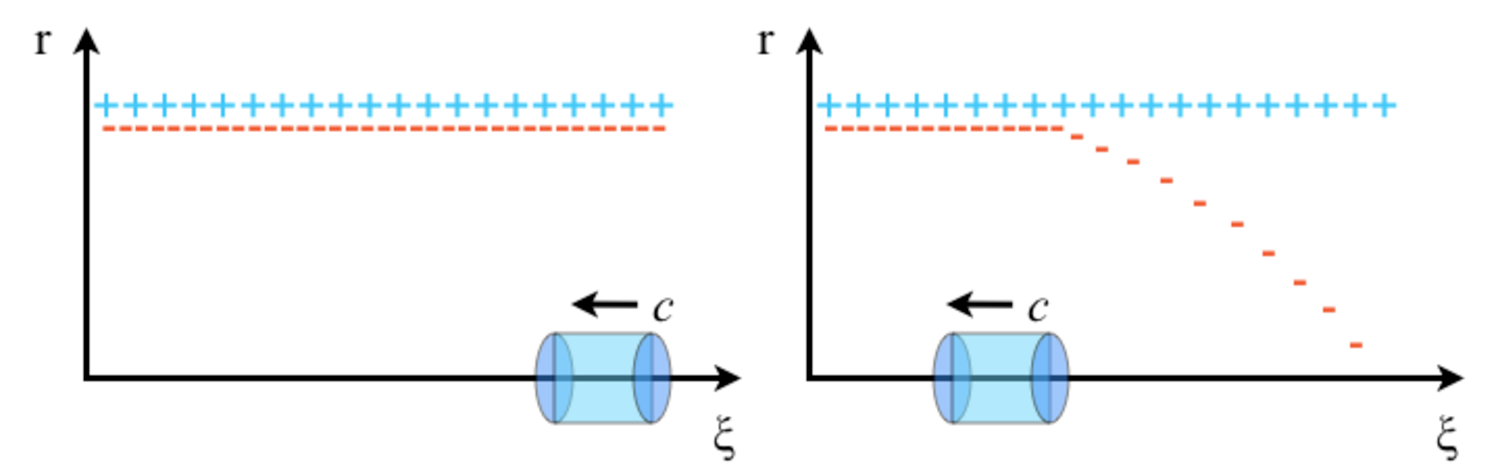
\includegraphics[width=150mm]{./figures/thin_cyl.pdf}
      \caption{A thin cylinder plasma with a flat top drive beam.}
\end{figure}

The beam is a flat top with radius $\sigma_r \ll a$, energy $\gamma$, and charge density $n_b$. The beam line charge is $\lambda_b = n_b \pi \sigma_r^2$ and the beam current is:

\begin{equation}\label{eq:I_beam}
I_b = \frac{Q_b}{\sigma_z}c = \frac{n_b \pi \sigma_r^2 \sigma_z}{\sigma_z}c = \lambda_b c
\end{equation}

We can normalize the beam current $I_b$ to the Alfven Current $I_A = m_e c^3/e$ so $\bar{I} = e I_b /m_e c^3$. The quantity $\bar{I} = e \lambda_b/m_e c^2$ is also called the Budker parameter $\nu$. 

Next, we find the beam field at the plasma radius $a$ using Gauss's law:

\begin{equation}\label{eq:E_beam}
E_b = \frac{2 \lambda_b}{a} = \frac{2m_e c^2}{e} \frac{\bar{I}}{a}
\end{equation}

An electron at the plasma radius receives an inward kick $\Delta p = F \Delta t = -e E_b \sigma_z/c$ where $\sigma_z$ is the bunch length. We want to describe the evolution of the plasma after the beam has passed and we also assume that the beam is short compared to the relevant length scale in this problem which is the plasma radius $a$. Let's take $\sigma_z = a/10$ to get:

\begin{equation}\label{eq:norm_kick}
\Delta p = -e \frac{2m_e c^2 \bar{I}}{e}\frac{\sigma_z/c}{a} = -\frac{m_e c \bar{I}}{5}
\end{equation}  

Of course it is completely arbitrary to choose $\sigma_z = a/10$, but this allows us to see that the strength of the kick is really controlled by the peak current and nothing else. 

%We also note that our model does not include radiative effects, so for our model to be reasonably accurate, we should require that the normalized kick $\Delta p/m_e c \ll 1$ which means $\bar{I} \ll 5$. At FACET, $\bar{I} \approx 1$ and $\sigma_z/\lambda_p \approx 1/5$. 

We assume the ions are stationary. Even though the plasma cylinder is infinitely thin, we can still introduce a notion of charge shielding by noting that the amount of plasma electrons that participate in the interaction is proportional to the line charge of the beam $\lambda_b = m_e c^2 \bar{I}/e$. Then the plasma line charge interacting with the beam is:

\begin{equation}\label{eq:part_charge}
\lambda_i = \left\{ \begin{array}{lr}
m_e c^2 \bar{I}/e & \lambda_b < \lambda_0 \\
\lambda_0 & \lambda_b > \lambda_0
\end{array} \right.
\end{equation}

At this point our analysis branches. There are four regimes we will investigate in the thin cylinder model. They are

\begin{itemize}
\item $\lambda_b > \lambda_0$, small initial kick
\item $\lambda_b > \lambda_0$, large initial kick
\item $\lambda_b < \lambda_0$, small initial kick
\item $\lambda_b < \lambda_0$, large initial kick
\end{itemize}

We will define ``small initial kick" and ``large initial kick" rigorously later on. Qualitatively, a small initial kick means that the plasma electrons do not cross the beam axis and instead undergo small oscillations about the plasma ions at the cylinder radius. For a large initial kick the plasma electrons cross the beam axis. The on-axis $E_z$ field is much larger in this case.

The cases with $\lambda_b > \lambda_0$ are the simplest because in this scenario there is not enough charge in the plasma cylinder to shield the beam charge. All plasma electrons see the same force and behave coherently. We can use a particle model to describe the radial trajectory of the plasma electrons. The cases with $\lambda_b < \lambda_0$ are more complex because there is charge screening. The electrons do not all see the same force and the initially thin charge layer broadens. This case requires a fluid model to describe the full charge distribution $\rho(r,\xi)$.







\subsection{$\lambda_b > \lambda_0$, Small initial kick}

For the case $\lambda_b > \lambda_0$, all plasma electrons have the same radial position in the plasma sheath for all $\xi$. We seek an equation of motion for the position of the plasma electron sheath $r_s(\xi)$. To solve for $r_s$, we first need to solve for the potential $\psi$. The source term for $\psi(r,\xi)$ is $\rho - J_z$. Although the plasma sheath moves radially, no charge moves through the sheath so the radial current density $J_r = 0$. The continuity equation gives:

\begin{equation}\label{eq:cont2}
\frac{\partial}{\partial \xi}(\rho - J_z) = 0 \rightarrow \rho - J_z = const = \rho_0 
\end{equation}

We take the constant to be $\rho_0$ since before the beam arrives $J_z = 0$ and $\rho = \rho_0$ and this makes it easy to solve for $\psi(r)$ using Gauss's law. We choose to work with the plasma line charge density so

\begin{equation}\label{eq:rho_for_lamb}
\rho_0 = \frac{\lambda_0}{2 \pi r_s}\delta(r - r_s)
\end{equation}


We take $\psi(r=\infty) = 0$ because outside the cylinder, there is zero net charge (after the drive beam has passed), so Gauss's law gives $E_g(r > a) = 0$ and therefore $\psi(r > a) = const = 0$. Inside the electron sheath there is no charge either, so $E_g(r < r_s) = 0$ and $\psi(r < r_s) = \psi_0$. Between the electron sheath and the ion layer there is a net charge and Gauss's law gives $E_g(r) = 2\lambda_0/r$ for $r_s < r < a$. 

Actually, we do not need to confine ourselves to the case where $r_s < a$ (\emph{i.e.} the plasma electrons within the channel). If we want to consider oscillations of the plasma electrons about the ion cylinder we should also describe the field for $a <  r_s$. The field is $E_g(r) = -2\lambda_0/r$ for $a < r < r_s$  which is the same as in the previous case but the sign is flipped. We can accommodate both $r_s > a$ and $r_s < a$ in a single equation if we write:

\begin{equation}\label{eq:E_both}
E_g(r) = \frac{2\lambda_0}{r}\Theta(r-r_s) - \frac{2\lambda_0}{r}\Theta(r-a)
\end{equation}

$\Theta(r)$ is the Heaviside step function. Note that $\lambda_0 < 0$ refers to the plasma electron charge, so the first term in equation~\ref{eq:E_both} is the (negative) field due to the plasma electrons and the second term is the (positive) field due to the ions.

We can now find the potential by integrating the electric field:

\begin{equation}\label{eq:Psi_both}
\begin{array}{rcl}
\psi(r) & = & -\int_0^r E(r') dr' = \psi_0 - \int_{\min(r_s,a)}^r \frac{2\lambda_0}{r'}\left(\Theta(r-r_s) - \Theta(r-a)\right) dr' \\
& = & \psi_0 - 2\lambda_0\log\left(\frac{r}{r_s}\right)\Theta(r-r_s) + 2\lambda_0\log\left(\frac{r}{a}\right)\Theta(r-a)
\end{array}
\end{equation}

Using the boundary condition $\psi(\max(r_s,a)) = 0$ we find that $\psi_0 = 2\lambda_0 \log\left(\frac{a}{r_s}\right)$ for both $r_s < a$ and $r_s > a$. The sign of $\psi_0$ flips between cases. 

%\begin{figure}[ht]\label{fig:fields}
%  \centering
%    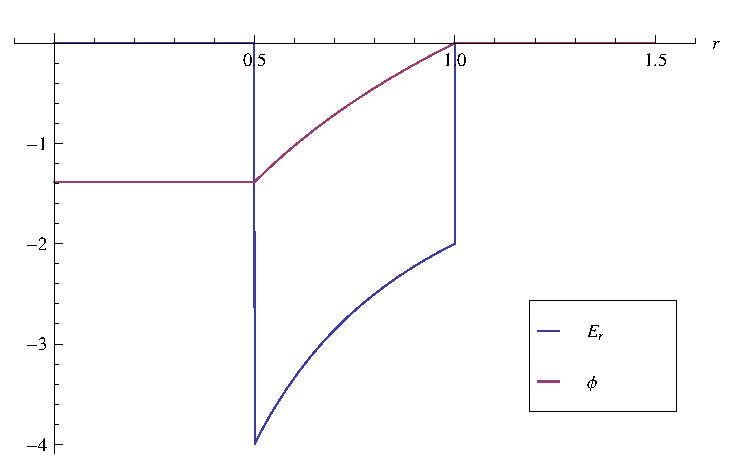
\includegraphics[width=100mm]{./figures/fields.pdf}
%      \caption{$E_g$ and $\psi$ for the thin cylinder model. $\bar{I} = 1$ and distances are normalized to $a=1$.}
%\end{figure}

\begin{figure}
\centering
\mbox{\subfigure{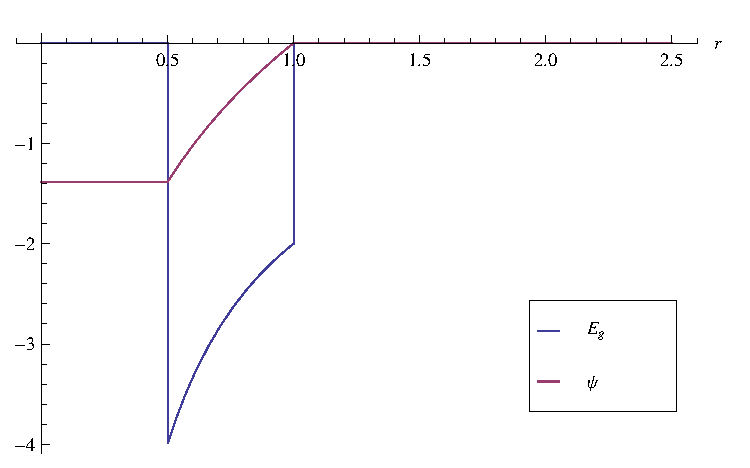
\includegraphics[width=3in]{./figures/fields_rs_small.pdf}}\quad
\subfigure{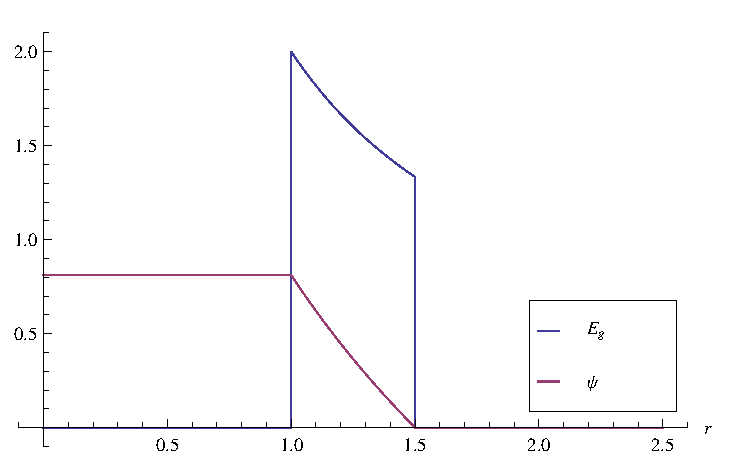
\includegraphics[width=3in]{./figures/fields_rs_large.pdf} }}
\caption{Left: $r_s = 0.5$, $a=1$. Right: $r_s = 1.5$, $a=1$.} \label{fig12}
\end{figure}

Next, we find $\mathbf{A}_{\perp}$ using equation~\ref{eq:gauge_qs}:

\begin{equation}\label{eq:a_perp}
\nabla_\perp \cdot \mathbf{A}_\perp = -\frac{\partial \psi}{\partial \xi} = - \frac{\partial \psi}{\partial r_s}\frac{\partial r_s}{\partial \xi}
\end{equation}

\begin{equation}\label{eq:dpsi}
\frac{\partial \psi}{\partial r_s} = \frac{2\lambda_0}{r_s}\Theta(r-r_s) + 2\lambda_0 \log\left(\frac{r_s}{r}\right)\delta(r-r_s) - \frac{2\lambda_0}{r_s} 
\end{equation}

%The second term in equation~\ref{eq:dpsi} is zero because the delta function forces the log to be evaluated at $r=r_s$. 

In cylindrical coordinates, the divergence is

\begin{equation}\label{eq:a_perp_cyl}
\nabla_\perp \cdot \mathbf{A}_\perp = \frac{1}{r}\frac{\partial}{\partial r} (r A_r) + \frac{1}{r}\frac{\partial A_{\theta}}{\partial \theta}
\end{equation}

but we drop the $\theta$ term due to the cylindrical symmetry. We note that $r$ and $r_s$ are independent variables in this equation so we can easily integrate the equation in $r$ to find $A_r$

\begin{equation}\label{eq:a_r}
A_r = -\frac{1}{r}\int_0^rr'\left[\frac{2\lambda_0}{r_s}\Theta(r'-r_s) + 2\lambda_0 \log\left(\frac{r_s}{r'}\right)\delta(r'-r_s) - \frac{2\lambda_0}{r_s}\right]\frac{\partial r_s}{\partial \xi}dr'
\end{equation}


%\begin{equation}\label{eq:a_r}
%\frac{1}{r}\frac{\partial}{\partial r} (r A_r) = -\frac{2\lambda_0}{r_s}r_s'\left[\Theta(r-r_s)-1\right] \rightarrow A_r = -\frac{\lambda_0 r r_s'}{r_s}\left[\Theta(r-r_s)-1\right] 
%\end{equation}

At this point, we'd like to start determining some physical quantities of interest, like $E_z$

\begin{equation}\label{eq:E_z}
E_z = \frac{\partial \psi}{\partial \xi} = \frac{2\lambda_0 r_s'}{r_s}\left[\Theta(r-r_s)-1\right] 
\end{equation}

This equation tells us three things. First, we see that $E_z$ is zero outside the plasma sheath away from the beam axis. Second, $E_z$ is independent of $r$ in this region (which is good).Third, $E_z$ is negative (at least in the first part of the oscillation) because the kick is inward $r_s' < 0$ and because $\lambda_0 < 0$. This makes sense because we expect the field to be decelerating for a positively charged driver. 

Now we need an equation of motion for $r_s$ which we can get by finding the force on the plasma electrons in the sheath:

\begin{equation}\label{eq:force}
F_r =-(E_r -v_z B_{\theta}) = \frac{\partial \phi}{\partial r} - v_z\frac{\partial A_z}{\partial r} + (1-v_z)\frac{\partial A_r}{\partial \xi}
\end{equation}

The second term on the right hand side of equation~\ref{eq:force} is the field due to the beam current which we neglect because we assume the beam has passed. Evaluating the remaining derivatives in~\ref{eq:force} we have:

\begin{equation}\label{dphi}
\frac{\partial \phi}{\partial r} = -\frac{2\lambda_0}{r}\left[\Theta(r-r_s)-\Theta(r-a)\right]
\end{equation}

\begin{equation}\label{dA_r}
\frac{\partial A_r}{\partial \xi} = -\frac{\lambda_0 r r_s''}{r_s}\left[\Theta(r-r_s)-1\right] + \frac{\lambda_0 r r_s'^2}{r_s^2}\left[\Theta(r-r_s)-1\right] + \frac{\lambda_0 r r_s'^2}{r_s}\delta(r-r_s)
\end{equation}

%We also note that $J_z = v_z \rho$ so in general we have:
%
%\begin{equation}\label{rho}
%\begin{array}{lr}
%\rho &= \frac{\rho_0}{1-v_z} \\
%J_z &= \frac{v_z\rho_0}{1-v_z}
%\end{array}
%\end{equation}



We need to evaluate the derivatives at the position of the electron sheath $r_s$. There is an ambiguity in the value of $\Theta(0)$. It can be 0, $1/2$, or 1 depending on your definition of $\Theta$. We can consider the three values the ``inside", ``on", and ``outside" trajectories of the electron sheath and calculate the field at $r=r_{s-}$,  $r=r_{s}$,  $r=r_{s+}$ with the respective values of $\Theta$.

\begin{equation}\label{eq:dphi_all}
\begin{array}{lcl}
\left.\frac{\partial \phi}{\partial r} \right|_{r=r_s-} & = & 0 \\
\left.\frac{\partial \phi}{\partial r} \right|_{r=r_s} & = & -\frac{\lambda_0}{r_s} \\
\left.\frac{\partial \phi}{\partial r} \right|_{r=r_s+} & = & -\frac{2\lambda_0}{r_s}
\end{array}
\end{equation}

\begin{equation}\label{eq:dA_r_all}
\begin{array}{lcl}
\left.\frac{\partial A_r}{\partial r} \right|_{r=r_s-} & = & \lambda_0 r_s'' - \frac{\lambda_0 r_s^2}{r_s} + \lambda_0 r_s'^2 \\
\left.\frac{\partial A_r}{\partial r} \right|_{r=r_s} & = & \frac{\lambda_0 r_s''}{2} - \frac{\lambda_0 r_s^2}{2 r_s} + \lambda_0 r_s'^2\\
\left.\frac{\partial A_r}{\partial r} \right|_{r=r_s+} & = & \lambda_0 r_s'^2
\end{array}
\end{equation}
%\begin{equation}\label{eq:E_r}
%E_r =-\nabla_{\perp} \phi - \frac{\partial A_r}{\partial \xi} = \frac{\bar{I} r}{r_s^2}[r_s r_s'' - r_s'^2]
%\end{equation}

%with $\nabla_{\perp} \phi = 0$ for the sheath electrons because there is zero charge within the sheath layer. 

The equation of motion is: 

\begin{equation}\label{eq:EOM_1}
\frac{\partial P_\perp}{\partial \xi} = \frac{1}{1-v_z} F_r
\end{equation}

It is easiest to solve this equation for $r=r_{s-}$ because in that case $\partial_r \phi = 0$ and the $(1-v_z)^{-1}$ drops out. We rewrite the EOM with the ``particle tracking" trajectory $\xi = t - z \rightarrow \partial_{\xi} = (1-v_z)\partial_t$:

\begin{equation}\label{eq:track}
\frac{\partial P_{\perp}}{\partial \xi} = \frac{\partial \gamma v_{\perp}}{\partial \xi} =  \frac{\partial}{\partial \xi}\left(\gamma \frac{\partial r_{\perp}}{\partial t}\right) = \frac{\partial}{\partial \xi}\left[\gamma (1-v_z)\frac{\partial r_{\perp}}{\partial \xi}\right]
\end{equation}

and using the integral of motion $\gamma - P_z = 1 + \psi$

\begin{equation}\label{eq:EOM_2}
\left. \frac{\partial P_{\perp}}{\partial \xi}\right|_{r=r_s-} = \left. \frac{\partial}{\partial \xi}[(1+\psi)r_s'] \right|_{r=r_s-}= \lambda_0\left[r_s'' +\frac{r_s'^2}{r_s}(r_s-1)\right]
\end{equation}

Plugging in $\psi$ and taking the derivative we have we have:

\begin{equation}\label{eq:rs}
\left(1-2\lambda_0\log\left(\frac{r_s}{a}\right) \right)r_s'' -\frac{\lambda_0 r_s'^2}{r_s} = \lambda_0\left[r_s'' +\frac{r_s'^2}{r_s}(r_s-1)\right]
\end{equation}

In order to study this equation, let's set $a=1$:

\begin{equation}\label{eq:rs_simp}
[1-\lambda_0(1+2\log(r_s))] r_s'' - \lambda_0 r_s'^2\left(\frac{1}{r_s}+1\right) = 0
\end{equation}


%\begin{figure}[ht]\label{fig:sheath}
%  \centering
%    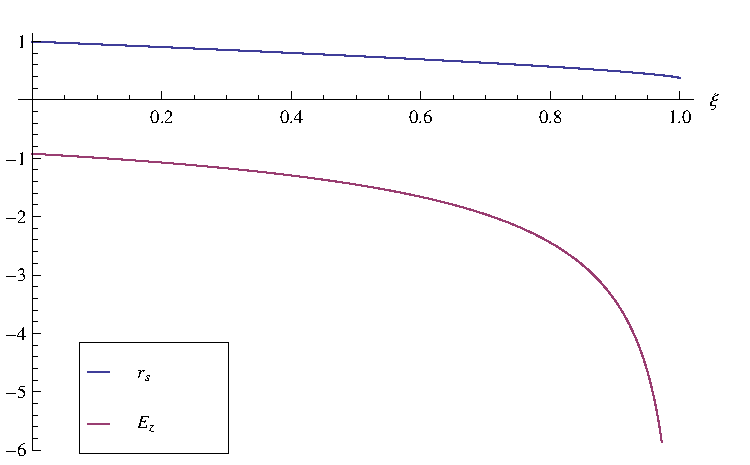
\includegraphics[width=100mm]{./figures/sheath.pdf}
%      \caption{$r_s$ and $E_z$ for the thin cylinder model. $\bar{I} = 1$ and distances are normalized to $a=1$. The initial kick $r_s'(0) = -0.46$. This is the largest kick that %Mathematica can use to solve the equation for the given plot range.}
%\end{figure}



\end{document}